\chapter{Preparation}

This chapter explain preparation undertaken when analysing the requirement of the project as well as acquiring knowledge necessary to ensure timely completion of its goals. I also aim to explain some design decisions made along the way and their effect on the final outcome of this project.

\section{Research}

In my project I set out to explore existing tools for sentiment analysis and apply them to the problem of classifying multilingual tweets. It was clear from the onset of the project that I need to carefully choose which utilities or libraries to use as I was gearing towards exposing the results of my analysis through and API and a web application.

Research has therefore been made into not only existing toolkits such as WEKA, but also lower level libraries (in particular libsvm and SVM$^{light}$) which would later enable me to easily run the classifiers in the context of a web application.

\section{Language Choice}

I set out not only to evaluate existing solutions to sentiment classification across different languages but also lay foundations for a platform which can later be turned into a web application and an API. There are certain languages which are particularly well-suited for this purpose, such as  Python, Ruby or PHP. All these languages have bindings to lower-level classification libraries, but Ruby in particular stood out by having a set of tools well-geared towards building scalable APIs, such as Rack\footnote{\url{http://rack.rubyforge.org/}} and Sinatra \footnote{\url{http://www.sinatrarb.com/}}. Similarly hosting platforms such as Heroku\footnote{\url{http://heroku.com}} make Ruby applications very easy to scale.

\section{Planning}

Planning and preparation are amongst factors significantly contributing towards a project's success. Moreover, little experience in Natural Language Processing (and machine learning techniques in particular) as well as the limited timescale of the project made it particularly ambitious.

I therefore needed to quickly verify my preconceptions and adopt to any unforeseen circumstances I might encounter along the way.

In order to do this efficiently, it was clear that I needed to build upon existing libraries and modify them only to the extent required by the scope of this project. Consideration also needed to be given to performance and scalability of the system, given it was planned to operate on a large data set in the future.

\section{Project Management}

In order to maintain flexibility of pursuing different paths in an area that is relatively new to me, I decided that a lightweight management approach such as Agile Software Development\footnote{\url{http://en.wikipedia.org/wiki/Agile_software_development}} would be appropriate for this project, which has therefore been divided into a number of iterations, each containing individual goals that should be met before progressing onto the next one (see Figure \ref{fig:iterative}). These are referred to in the Project Plan as `Weeks' and allow for identifying problems with missing deadlines early on in the project.

I tried to follow many of the principles outlined by Andrew Hunt is his book, The Pragmatic Programmer\cite{PragProg}, in which he offers an approach to software design which allows for developing and delivering high-quality software products.

\begin{figure}[htb]
  \begin{center}
    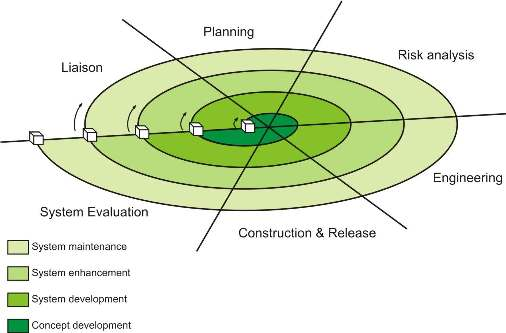
\includegraphics[width=0.8\textwidth]{iterative.jpg}
    \caption{Illustration of an agile development process}
    \label{fig:iterative}
  \end{center}
\end{figure}

Multiple factors were taken into account when establishing project milestones and their respective deadlines:

\begin{itemize}
  \item Sufficient knowledge of Twitter API and a familiar development environment need to be established before any other work can be commenced.
  \item Preliminary data set needs to be gathered within first four weeks of the project in order to ensure evaluation work, even if limited, can be carried out.
  \item Evaluation and implementation chapters shall be written as subsequent classifiers are implemented.
  \item All classifiers shall be implemented before Easter Vacation.
  \item All chapters of the dissertation shall be written before the 2nd of May to allow for revision before exams.
\end{itemize}

This division was made possible by the modular nature of the project.

\section{Tools Used}

In order to avoid potential data loss and subsequent failure to meet the deadlines established in the project plan, a number of tools are used to ensure all code and the dissertation itself is properly versioned and backed up.

All code (including {\LaTeX} source code for the dissertation itself) is stored in a version control system (git\footnote{\url{http://git-scm.com/}}). The repository is mirrored to GitHub\footnote{\url{http://github.com}} and further backups are stored on Dropbox\footnote{\url{http://dropbox.com}} and my personal Time Capsule\footnote{\url{http://www.apple.com/timecapsule/}} to further mitigate any risk of data loss.

This provides a level of redundancy sufficient to finalise the project within desired timeline.

\section{Data Sources}

We use Twitter as our primary data source, primarily because it offers the biggest freely accessible source of real-time status updates.
There are however some characteristics of Twitter messages that need to be taken into account when designing our experiments and evaluating their results.

\begin{itemize}
  \item \textbf{Length.} Twitter messages are explicitly limited to 140 characters. Our dataset contains tweets which are 57 characters or 9 words long on average. It is interesting to note that the average length of a Twitter message seems to have fallen compared what has been shown in previous research \cite{TwitterDistantSupervision09} from 2009, where an average tweet was 78 characters (or 14 words) long. This can be attributed to sharing of links becoming a more prominent use case of Twitter.
  \item \textbf{Language model.} Twitter messages often contain slang, misspelling or even colloquially used phrases borrowed from different languages (English in particular).
  \item \textbf{Domain.} Twitter messages have a very diversified domain and are not centred about any particular topic.
\end{itemize}

Availability of tweets in different languages was also a concern. Due to both the limitations of the Twitter API as well as some languages being more likely to appear that the other, I needed to make provisions in case this process took longer than anticipated.

\section{Algorithms}

This section outlines mathematical models behind algorithms I used for sentiment classification.

\subsection{Feature Selection}

Different approaches can be taken when selecting features to be fed into classification algorithms. Some of the libraries outlined in the Available Tools section offer built-in feature extraction capabilities (including Porter stemming).

As shown by A. Go et al. \cite{TwitterDistantSupervision09}, there is little to be gained from going beyond the simplest unigram model. Therefore, for the purpose of this project we shall assume that each feature is a single word found in a tweet. Additionally, a number of feature reduction techniques described in the following chapter are employed in order to reduce the feature space.

\subsection{Na\"ive Bayes}

Na\"ive Bayes is a simple classifier based on applying Bayes' Theorem, often used for robust document classification due to its simplicity. One of its advantages is that it requires relatively small amount of training data before achieving peak performance.

In our model, a simple Bayesian classifier can be represented as a function mapping features ($f_1{\ldots}f_n$) to a class ($c$) which is which this combination of features is most likely:

$$\mathrm{classify}(f_1,\dots,f_n) = {\mathrm{argmax}} \ P(C=c) \prod_{i=1}^n P(F_i=f_i\vert C=c).$$

It is important to note that if we allow $P(F_i=f_i\vert C=c)$ to be equal to $0$ (such as when our test vector contains features not present in the training data), the probability of that data point being in any class will also equal $0$, irrespective of the likelihood of other features.

To avoid this phenomenon, we shall use \emph{add-one} or \emph{Laplace smoothing}, where we assume that all features, including unsed ones, are initialised with a count of $1$.

\subsection{Maximum Entropy}

Maximum Entropy is a group of feature-based models which do not assume independence of features, unlike Bayesian classifiers. In our simplified, unigram-based approach, this provides little benefit as features do not overlap. Additional complexity makes MaxEnt slower in comparison to Na\"ive Bayes, imposing additional limitations given our attempt to keep scalability in mind.

Maximum Entropy can also suffer from overfitting when training data is too sparse. In order to improve performance, we shall integrate a Gaussian prior by using maximum a posteriori estimation instead of maximum likelihood. This is incorporated natively in the library that I use in this project.

\subsection{Support Vector Machines}

Support Vector Machines are a set of supervised learning methods which can be used as a non-probabilistic binary linear classifier by constructing a set of hyperplanes in a high or infinite dimensional space with the class assigned to new data points being dependent on their location in that space.

This model can be formalised by assuming we have a set of training data $\mathcal{D}$ and a set of $n$ points of the form

$$\mathcal{D} = \left\{ (\mathbf{x}_i, y_i)\mid\mathbf{x}_i \in \mathbb{R}^p,\, y_i \in \{-1,1\}\right\}_{i=1}^n$$

where $y_i$ denotes the class to which point $x_i$ belongs. We can now define any hyperplane as a set of points $\mathbf{x}$ satisfying the following

$$\mathbf{w} \cdot \mathbf{x} - b = 0$$

where $\mathbf{w}$ is a normal vector, where $\frac{b}{||\mathbf{w}||}$ determines the offset of given hyperplane along the normal vector $\mathbf{w}$.

Now in order to separate data into classes we define two further hyperplanes described by the equations

$$\mathbf{w} \cdot \mathbf{x} - b = -1$$

and

$$\mathbf{w} \cdot \mathbf{x} - b = 1$$

and try to find $\mathbf{w}$ and $b$ to maximise the distance between parallel hyperplanes so that they are as far apart as possible whilst still separating the data. For an illustration see Figure \ref{fig:svm}.

\begin{figure}[htb]
  \begin{center}
    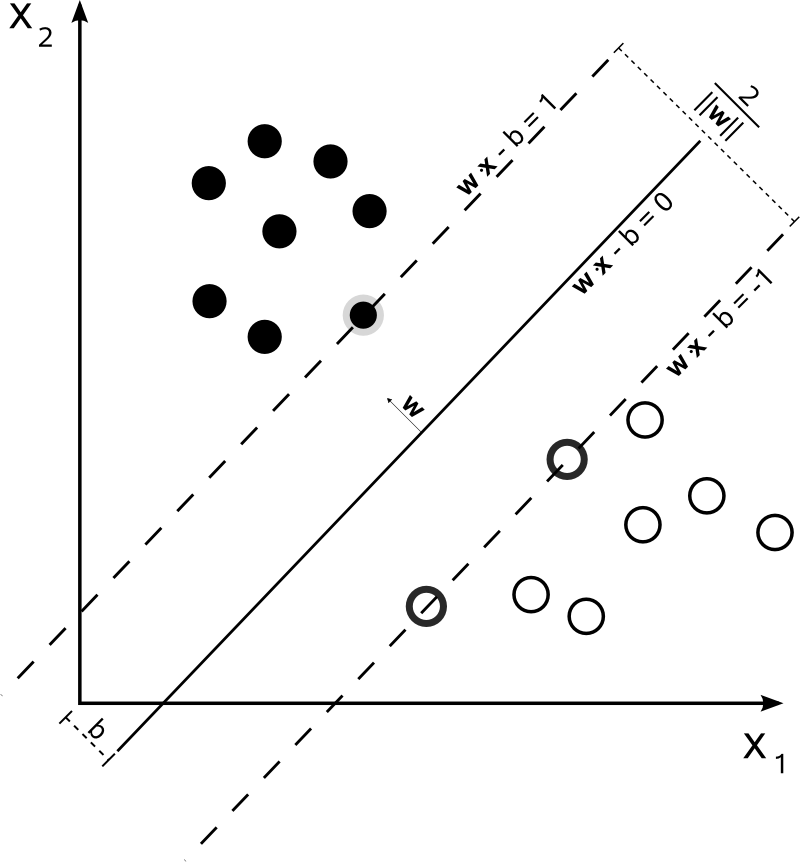
\includegraphics[width=0.8\textwidth]{svm.png}
    \caption{Maximum-margin hyperplane and margins for an SVM trained with samples from two classes -- Wikipedia}
    \label{fig:svm}
  \end{center}
\end{figure}

\section{Available Tools}

This section explores existing tools for sentiment classifications and describes the rationale behind selecting those which had been used for this project. 

\subsection{Na\"ive Bayes}

The simplicity of Na\"ive Bayes classification means it is one of the most commonly implemented techniques in any machine learning package. It is therefore easy to find libraries that implement this particular classifier. Amongst the ones I explored were \verb|WEKA|\footnote{\url{http://www.cs.waikato.ac.nz/ml/weka/}}, \verb|Orange|\footnote{\url{http://orange.biolab.si/}} and \verb|Classifier4J|\footnote{\url{http://classifier4j.sourceforge.net/}}.

Both \verb|WEKA| and \verb|Orange| are GUI machine learning toolkits for data analysis and predictive modelling, particularly useful in research where there are few time and scalability concerns. I found them useful learning tools to experiment with different classification methods, but in order to meet the requirements of this project, a scalable lower-level solution was needed.

\verb|Classifier4J| meets most of these criteria, but due to limited documentation and lack of activity in the project since 2005 I abandoned it in favour of a more modern solution.

In the end I settled on a Ruby library \verb|Ankusa|, which due to its support for Hadoop's \verb|HBase|\footnote{\url{http://hbase.apache.org/}} and \verb|Cassandra|\footnote{\url{http://cassandra.apache.org/}} for storage offered promising scaling capabilities. My familiarity with Ruby has also proven helpful in understanding the internals of the library and enabled me to modify it to the extent required by this project.

\subsection{Maximum Entropy}

Unfortunately there are very few libraries Ruby libraries that implement Maximum Entropy classifiers. Initially, attempts were made to use \verb|maxent|\footnote{\url{http://mastarpj.nict.go.jp/~mutiyama/software.html\#maxent}}, which had proven difficult given lack of documentation and updates since 2008 (since then Ruby 1.9.x became standard and many 1.8.x libraries stopped working).

In the end I decided to use \verb|maxent_string_classifier|\footnote{\url{https://github.com/mccraigmccraig/maxent_string_classifier}}, which is based on the \verb|OpenNLP|\footnote{\url{http://incubator.apache.org/opennlp/}} \verb|Maxent| framework. The library is well-maintained and has reasonably comprehensive documentation. The only disadvantage of using \verb|maxent_string_classifier| is that it introduces a dependency on JRuby\footnote{\url{http://www.jruby.org/}}, which is a Java implementation of the Ruby programming language.

\subsection{Support Vector Machines}

Having been warned on multiple occasions that Support Vector Machines might be difficult to integrate, I decided to research them ahead of schedule to avoid any potential delays. I looked into GUI tools such as \verb|WEKA|, but none of them have the scaling properties required to parse a large number of messages in real time.

After thorough considerations, \verb|libsvm|\footnote{\url{http://www.csie.ntu.edu.tw/~cjlin/libsvm/}} and \verb|Eluka|\footnote{\url{https://github.com/arrac/eluka}} were chosen as they seemed to meet my performance requirements whilst remaining relatively easy to use.

\section{Verification}

This project makes a number of assumptions regarding the training data set that needed to be verified manually in order to establish confidence of results presented. Firstly, we assumed that Twitter's built-in language filter works reliably, for which there was no evidence by either Twitter or any third parties. Secondly, it is difficult to determine the actual sentiment of a tweet because of humour, sarcasm and non-standard use of emoticons, potentially rendering our assumption that they can be used as labels for training data unfounded.

Since manual verification would require access to a number of people fluent in five different languages evaluated in this project, I first attempted to find a solution which would make this process easier.

In my preliminary research, Amazon Mechanical Turk\footnote{\url{https://www.mturk.com/}} seemed to be the forerunner in providing on-demand, scalable workforce for simple tasks such as manual classification of data. This solution was however quickly discarded as becoming a requester on the platform requires a US billing address.

I then shifted my focused to companies and tools which act as intermediaries between researches and Amazon's Mechanical Turk. This lead me to exploring and subsequently settling on CrowdFlower\footnote{\url{http://crowdflower.com/}}, which allows for publishing jobs not only to AMT but also other crowdsourcing platforms. It also offers an internal interface should any of the providers fail to complete requested tasks.

\section{Summary}

In this section I described the research undertaken in order to successfully plan the project and gather information about various machine learning techniques and their applications in the area of sentiment classification. I also discussed how my assumptions regarding the use of emoticons and Twitter's built-in language filter will be verified.